% !TeX program = pdflatex
\documentclass[tikz,border=8pt]{standalone}
\usepackage{tikz}
\definecolor{FigureBlue}{HTML}{2563EB}
\begin{document}
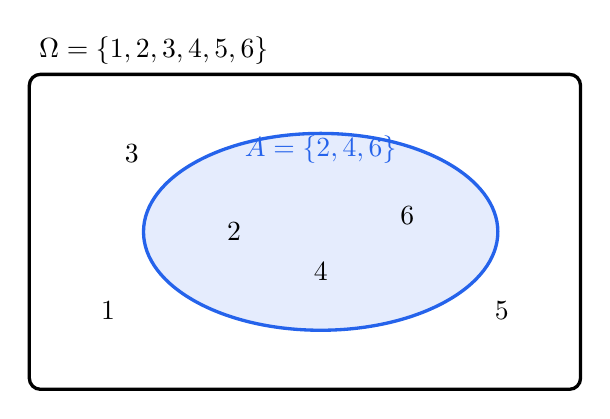
\begin{tikzpicture}
  \draw[rounded corners,line width=1.2pt] (0,0) rectangle (7,4); \node[above right] at (0,4) {$\Omega=\{1,2,3,4,5,6\}$};
  \draw[FigureBlue,fill=FigureBlue!12,line width=1.2pt] (3.7,2) ellipse (2.25 and 1.25); \node[FigureBlue] at (3.7,3.05) {$A=\{2,4,6\}$};
  \node at (1,1) {$1$}; \node at (1.3,3) {$3$}; \node at (6,1) {$5$};
  \node at (2.6,2) {$2$}; \node at (3.7,1.5) {$4$}; \node at (4.8,2.2) {$6$};
\end{tikzpicture}
\end{document}
